\documentclass[a4paper,11pt]{article}

\usepackage[spanish]{babel}
\usepackage[utf8]{inputenc}
\usepackage{enumerate}
\usepackage{amsmath}
\usepackage{extsizes}
\usepackage{amssymb}
\usepackage{dsfont}
\usepackage{graphicx}
\usepackage{cancel}
\usepackage[usenames]{color}
\usepackage[dvipsnames]{xcolor}
\usepackage{accents}
\usepackage{flushend}
\usepackage{tikz}
\usepackage[LGR,T1]{fontenc}
\newcommand{\textgreek}[1]{\begingroup\fontencoding{LGR}\selectfont#1\endgroup}
\usetikzlibrary{arrows,automata}
\usepackage{multicol}
\setlength{\columnsep}{1cm}
\usepackage{listings}
\usepackage{graphics,graphicx, float} %para incluir imágenes y colocarlas



\usepackage[hidelinks]{hyperref}

\usepackage[vmargin=3cm,hmargin=3cm]{geometry}
%\setlength\parindent{0pt}

\setlength\parindent{0pt}


% Carpeta con las imágenes
%\graphicspath{{}}

\begin{document}


	\begin{center}
		\LARGE{\textbf{Nuevos Paradigmas de Interacción (2018-2019)} \\ Grado en Ingeniería Informática \\ Universidad de Granada }
		\vspace*{2.5cm}

		\rule{\textwidth}{1.6pt}\vspace*{-\baselineskip}\vspace*{4pt}
		\rule{\textwidth}{1.6pt}\vspace*{-\baselineskip}\vspace*{2pt}
		\vspace{0.5cm}

		\Huge{Memoria Técnica}

		\vspace{0.5cm}
		\rule{\textwidth}{1.6pt}\vspace*{-\baselineskip}\vspace*{2pt}
		\rule{\textwidth}{1.6pt}\vspace*{-\baselineskip}\vspace*{4pt}

		\vspace{2cm}

\begin{figure}[h!]
	\centering
	
\includegraphics[scale=1]{./Imagenes/logo_informatica.png}
	\label{fig:logougrciencias}
\end{figure}

		\vspace{4cm}
		\LARGE{Ignacio Aguilera Martos, Diego Asterio de Zaballa,\\ Manuel López Roldán \\ 16 de Diciembre de 2018 }

	\end{center}




\newpage

\tableofcontents

\newpage

\section{Idea, dispositivo y plataforma de desarrollo}

El proyecto que hemos querido desarrollar para la tercera práctica con integración de gestos es una continuación de nuestra idea de las dos primeras prácticas. Esta idea era la integración de un museo virtual lleno de cuadros a los que ahora se le suman modelos en 3D tales como esculturas o edificios que son manejados mediante gestos leídos con el dispositivo Leap Motion.

\vspace{10px}

El dispositivo escogido ha sido Leap Motion ya que es un dispositivo cuyo último SDK está pensado y desarrollado para la integración con las gafas de realidad virtual con lo que la integración con nuestra aplicación sería muy coherente. El dispositivo iría pegado a las gafas de tal forma que el usuario puede realizar los gestos sin necesidad de colocarse en un punto concreto o encima de algún elemento concreto puesto que los gestos son leídos directamente desde el Leap que apunta siempre a las manos por su localización en las gafas de VR. En este sentido la aplicación aún no está preparada para poder comunicarse con el dispositivo móvil puesto que es el componente que falta por desarrollar por el equipo de desarrolladores de Leap Motion Inc. y que ya han anunciado que están trabajando en esta integración. De momento el Leap puede emplearse como lo hemos integrado nosotros, es decir desde el ordenador, con el cuál si tiene una integración gestual sólida.

\vspace{10px}

Cabe decir que la plataforma que hemos elegido para el desarrollo de la aplicación ha sido Unity 3D. Esta decisión viene motivada por la facilidad de uso que nos da este entorno de desarrollo en el ámbito tridimensional así como la fácil integración de Leap Motion y reconocimiento de los datos provistos por el dispositivo ya que sus desarrolladores han implementado un Asset de Unity para facilitar el manejo del mismo. La integración por tanto con nuestra anterior idea del museo sería muy sencilla puesto que ambos proyectos están implementados en Unity y por tanto sólo se necesitaría diferenciarlos en dos escenas que serían cargadas convenientemente en función de si se quieren visualizar los cuadros o los modelos 3D.

\vspace{10px}

Una vez explicado esto, para desarrollar mejor la idea del proyecto, vamos a dar una introducción más específica sobre lo implementado para luego desgranar los aspectos técnicos del mismo.

\section{Proyecto}

El proyecto nos muestra nuestras manos reconocidas por el Leap Motion para poder interactuar adecuadamente con los objetos y poder ver cuándo los estamos tocando. La primera pantalla que se nos muestra es un menú tridimensional que es accedido presionando las opciones tal y como se muestra en los proyectos de ejemplo del Leap Motion. El menú nos da las cuatro opciones que tenemos para poder navegar e interactuar con las esculturas del museo que son: Observation Mode, Free World Mode, Play Mode y Exit.
\begin{itemize}
	\item Observation Mode: El Observation Mode nos permite visualizar la estatua en 3D como un modelo que se presenta en el centro de la escena y con la cual podemos interactuar gestualmente para desplazarla como queramos o hacerle zoom.
	\item Free World Mode: Este modo es el que nos permitirá visualizar la escena con realidad aumentada una vez que el SDK de Leap Motion tenga disponible la comunicación entre el dispositivo y el propio spartphone.
	\item Play Mode: Con este modo tenemos disponible un mundo con físicas que nos permite interactuar con elementos como cubos o la propia estatua para poder jugar desplazando los elementos, manipulándolos o tirándolos.
	\item Exit: Nos permite salir de la aplicación.
\end{itemize}

A continuación vamos a detallar más la estructura general de la escena para poder entrar posteriormente más en profundidad en cada modo y los gestos desarrollados.

\section{Estructura de la escena}

Para comenzar vamos a visualizar un esquema de los nodos principales de la escena:

\begin{figure}[!h]
	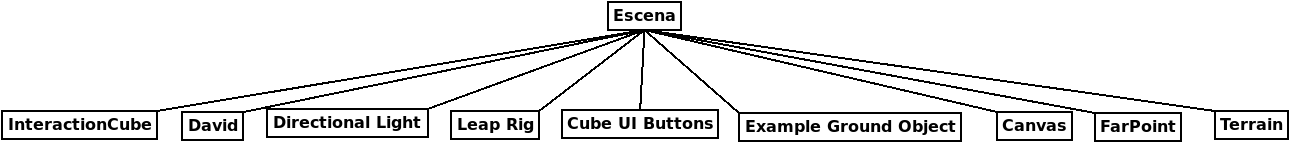
\includegraphics[scale=0.8]{./Imagenes/Escena.png}
	\caption{Diagrama de la escena principal}
	\label{escena}
\end{figure}

Como podemos observar la escena contiene 9 elementos en total que vamos a explicar a continuación:

\begin{itemize}
	\item InteractionCube, FarPoint, Terrain y David: estos elementos son los que componen el modelo tridimensional del David de Miguel Ángel (estatua que se muestra en nuestra aplicación). Este conjunto hace que tengamos una hitbox con la que interactuar con el modelo así como un terreno para prevenir de que desaparezca de la escena. Este último elemento es empleado cuando activamos el Play Mode ya que las figuras de la escena ganan propiedades de físicas con lo que podemos interactuar con ellos y para lo que necesitamos un plano inferior que nos haga de suelo para que la gravedad no se lleve los elementos hacia abajo indefinidamente.
	\item Directional Light: este elemento de la escena nos da la forma en la que la luz se aplica sobre la escena. Es el objeto que provee de una fuente de luz a la misma.
	\item Leap Rig: este elemento de la escena es el que contiene la funcionalidad y las características del Leap Motion así como la recopilación de los datos del mismo para que posteriormente se puedan utilizar en nuestro script de detección de gestos. Viene incorporado en el Asset provisto por los desarrolladores de Leap Motion Inc. para Unity.
	\item Cube UI Buttons: este elemento incorpora los botones con los que se puede interactuar mediante las manos virtuales de las que nos provee el SDK de Leap Motion.
	\item Canvas: en este nodo del gafo de la escena tenemos los textos que se incorporan en los botones para poder distinguirlos entre sí de forma visual.
\end{itemize}

No sólo tenemos estos elementos dentro de la escena, si no que también hay algunos nodos que contienen subnodos relevantes en el desarrollo del proyecto y de los cuales haremos una breve explicación para exponer su utilidad dentro del mismo.

\vspace{10px}

En primer lugar explicaremos el árbol que obtenemos del nodo Leap Rig:

\begin{figure}[!h]
	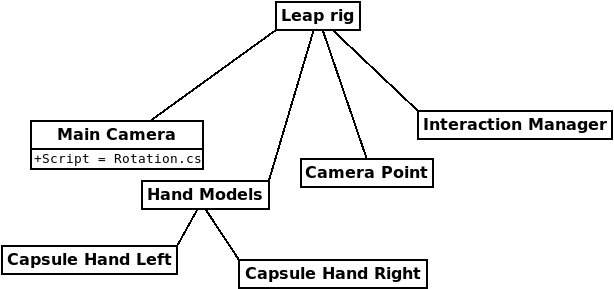
\includegraphics[scale=0.75]{./Imagenes/Leap_Rig.png}
	\caption{Diagrama del nodo Leap Rig}
	\label{leapRig}
\end{figure}

\begin{itemize}
	\item Main Camera y Camera Point: estos elementos representan la cámara de la escena, esto es, dónde estará por defecto el usuario y que le permitirá cambiar el foco de atención a diferentes zonas de la misma si lo requiere. Sobre estos elementos de la escena es sobre los que se coloca el script Rotation.cs que es el que contiene el código referente a los gestos implementados y que posteriormente explicaremos.
	\item Hand Models: Estos elementos son los que implementan el modelo tridimensional de las manos que interactúa y se mueve con respecto a las nuestras mediante el dispositivo Leap Motion. Gracias a estos modelos la experiencia del usuario es mucho más fácil ya que así tiene una percepción real de dónde están sus manos virtuales en la escena.
	\item Interaction Manager: Este componente contiene el procesamiento de la información de las manos mediante el Leap e integra la compatibilidad con VR para Oculus y HTC Vive. Dentro de este objeto tenemos un interactuador para cada mano que recoge la información sobre cada dedo (si está o no extendido), sobre la velocidad de cada mano y sobre el vector de dirección y el vector normal de la palma de la mano. Esta información será accedida posteriormente para la elaboración de los gestos.
\end{itemize}

\vspace{20px}

También tenemos elementos en el nodo Cube UI Buttons los cuales son los propios botones para cada opción.

\begin{figure}[!h]
	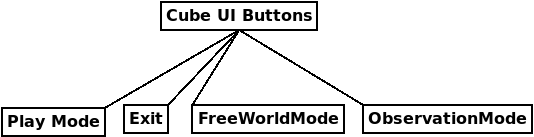
\includegraphics[scale=0.8]{./Imagenes/Cube_UI_Buttons.png}
	\caption{Diagrama de Cube UI Buttons}
	\label{cubeUIButtons}
\end{figure}

Cada uno de estos botones contiene un objeto de tipo Button Cube que son los botones con los que Leap puede interactuar presionándolos y que vienen incluidos en el Asset de Leap Motion.

\vspace{10px}

Asimismo tenemos que del nodo Canvas cuelgan los textos que se superponen sobre los botones.

\begin{figure}[!h]
	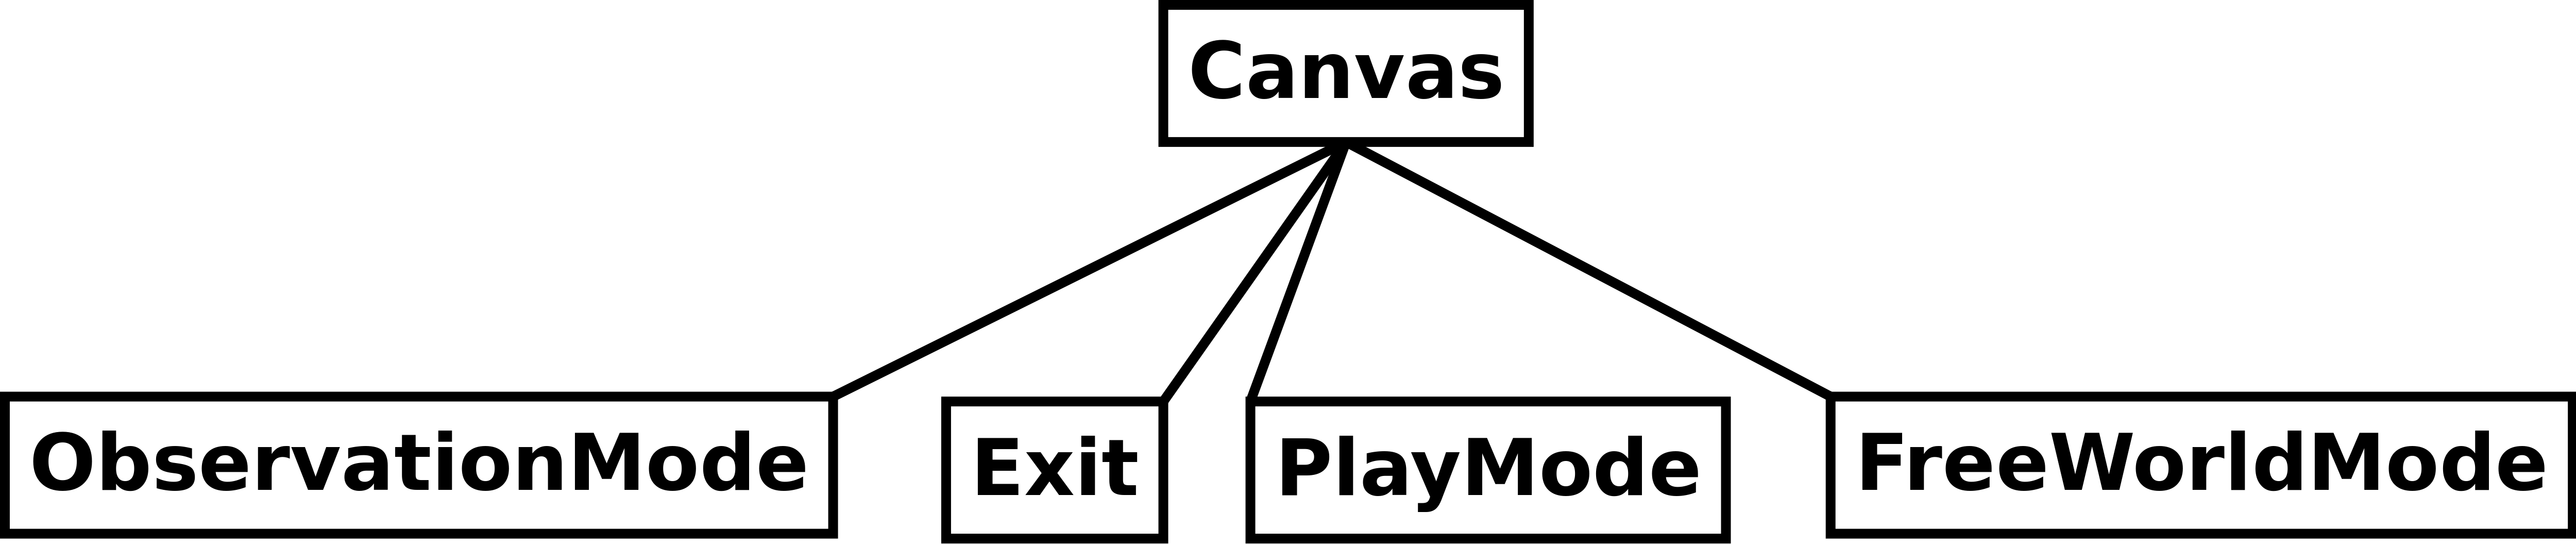
\includegraphics[scale=0.7]{./Imagenes/Canvas.png}
	\caption{Diagrama del nodo Canvas}
	\label{canvas}
\end{figure}

Estos textos se enlazan al botón correspondiente del nodo Cube UI Buttons.

\end{document}
